\documentclass[10pt,a4paper]{article}

\usepackage[english]{babel}

\usepackage[margin=22mm]{geometry}
\usepackage{amsmath,amsthm,amssymb,scrextend,graphicx,ifthen,hyperref}
\usepackage{fancyhdr}
\pagestyle{fancy}

\usepackage{listings}

\usepackage{algorithmic}
%\usepackage{algpseudocode}
\usepackage{mdframed}

\usepackage{float}

\usepackage{tcolorbox}
\usepackage{tikz}
\usepackage{todonotes}

\usepackage{pgfplots,pgfplotstable}
\pgfplotsset{compat=1.15}

\usepackage[small,compact]{titlesec}
\titlespacing{\section}{0pt}{2ex}{1ex}
\titlespacing{\subsection}{0pt}{1ex}{0ex}
\titlespacing{\subsubsection}{0pt}{0.5ex}{0ex}
\setlength{\parskip}{0cm}
\setlength{\parindent}{1em}

\newcommand{\N}{\mathbb{N}}
\newcommand{\Z}{\mathbb{Z}}
\newcommand{\I}{\mathbb{I}}
\newcommand{\R}{\mathbb{R}}
\newcommand{\F}{\mathbb{F}}
\newcommand{\C}{\mathbb{C}}
\newcommand{\Q}{\mathbb{Q}}
\renewcommand{\qed}{\hfill$\blacksquare$}
\renewcommand{\Re}{Re}
\let\newproof\proof
\renewenvironment{proof}{\begin{addmargin}[1em]{0em}\begin{newproof}}{\end{newproof}\end{addmargin}\qed}
% \newcommand{\expl}[1]{\text{\hfill[#1]}$}

\theoremstyle{plain}
\newtheorem{theorem}{Theorem}
\newtheorem{proposition}[theorem]{Proposition}
\newtheorem{lemma}[theorem]{Lemma}
\newtheorem{corollary}[theorem]{Corollary}
\newtheorem{claim}[theorem]{Claim}
\newtheorem{problem}{Problem}

\theoremstyle{definition}
\newtheorem{definition}[theorem]{Definition}
\newtheorem{example}[theorem]{Example}
%\newtheorem*{comment}{Comment}

\newtheorem{remark}[theorem]{Remark}

\DeclareMathOperator{\epi}{epi}
\DeclareMathOperator{\Span}{span}
\DeclareMathOperator{\Range}{range}
\DeclareMathOperator{\Null}{null}
\DeclareMathOperator{\argmin}{arg\,min}


\newcommand{\eps}{\varepsilon}
%%% Norms etc.
\newcommand{\inner}[3][n]{\SwitchBracketsizeLeft{#1}\LeftBracketSize\langle#2,#3\SwitchBracketsizeRight{#1}\RightBracketSize\rangle}
\newcommand{\abs}[2][n]{\SwitchBracketsizeLeft{#1}\LeftBracketSize\lvert#2\SwitchBracketsizeRight{#1}\RightBracketSize\rvert}
\newcommand{\norm}[2][n]{\SwitchBracketsizeLeft{#1}\LeftBracketSize\lVert#2\SwitchBracketsizeRight{#1}\RightBracketSize\rVert}
\newcommand{\set}[3][b]{\SwitchBracketsizeLeft{#1}\LeftBracketSize\{#2:#3\SwitchBracketsizeRight{#1}\RightBracketSize\}}

\newcommand{\NextScriptStyle}[1]{{\scriptstyle{#1}}}
\newcommand{\NextScriptScriptStyle}[1]{{\scriptscriptstyle{#1}}}
\newcommand{\NextTextStyle}[1]{{\textstyle{#1}}}
\newcommand{\NextDisplayStyle}[1]{{\displaystyle{#1}}}
\newcommand{\SwitchBracketsizeLeft}[1]{
  \ifthenelse{\equal{#1}{b}\OR\equal{#1}{big}}{\let\LeftBracketSize=\bigl}{
    \ifthenelse{\equal{#1}{B}\OR\equal{#1}{Big}}{\let\LeftBracketSize=\Bigl}{
      \ifthenelse{\equal{#1}{g}\OR\equal{#1}{bigg}}{\let\LeftBracketSize=\biggl}{
    \ifthenelse{\equal{#1}{G}\OR\equal{#1}{Bigg}}{\let\LeftBracketSize=\Biggl}{
      \ifthenelse{\equal{#1}{s}\OR\equal{#1}{small}}{\let\LeftBracketSize=\NextScriptStyle}{
        \ifthenelse{\equal{#1}{ss}}{\let\LeftBracketSize=\NextScriptScriptStyle}{
          \ifthenelse{\equal{#1}{t}\OR\equal{#1}{text}}{\let\LeftBracketSize=\NextTextStyle}{
        \ifthenelse{\equal{#1}{d}\OR\equal{#1}{display}}{\let\LeftBracketSize=\NextDisplayStyle}{
          \ifthenelse{\equal{#1}{a}\OR\equal{#1}{auto}}{\let\LeftBracketSize=\left}{
            \let\LeftBracketSize=\relax}}}}}}}}}}
\newcommand{\SwitchBracketsizeRight}[1]{
  \ifthenelse{\equal{#1}{b}\OR\equal{#1}{big}}{\let\RightBracketSize=\bigr}{
    \ifthenelse{\equal{#1}{B}\OR\equal{#1}{Big}}{\let\RightBracketSize=\Bigr}{
      \ifthenelse{\equal{#1}{g}\OR\equal{#1}{bigg}}{\let\RightBracketSize=\biggr}{
    \ifthenelse{\equal{#1}{G}\OR\equal{#1}{Bigg}}{\let\RightBracketSize=\Biggr}{
      \ifthenelse{\equal{#1}{s}\OR\equal{#1}{small}}{\let\RightBracketSize=\NextScriptStyle}{
        \ifthenelse{\equal{#1}{ss}}{\let\RightBracketSize=\NextScriptScriptStyle}{
          \ifthenelse{\equal{#1}{t}\OR\equal{#1}{text}}{\let\RightBracketSize=\NextTextStyle}{
        \ifthenelse{\equal{#1}{d}\OR\equal{#1}{display}}{\let\RightBracketSize=\NextDisplayStyle}{
          \ifthenelse{\equal{#1}{a}\OR\equal{#1}{auto}}{\let\RightBracketSize=\right}{
            \let\RightBracketSize=\relax}}}}}}}}}}


\newcounter{oppgave}

\newenvironment{oppgave}[1][]{\refstepcounter{oppgave}\par\medskip
 \noindent \textbf{Question~\theoppgave. #1} \rmfamily}{\medskip}

\newcounter{punkt}[oppgave]

\newenvironment{punkt}[1][]{\refstepcounter{punkt}\par\medskip
 \noindent \textbf{\theoppgave.\thepunkt. #1} \rmfamily}{\medskip}



\sloppy
\begin{document}

\lhead{SLIAL}
\chead{WS04: Linear optimization}
\rhead{\today}

\fancyfoot[R] {\thepage}
\fancyfoot[C] {}
\fancyfoot[L] {\small SEB, seb@livoni.me}
%\maketitle

\section*{Sparse solutions to linear algebraic systems}

In block 3 we dealt with \emph{overdetermined}/unsolvable systems of linear algebraic equations by reformulating them as the least squares problems.
Often, for example in machine learning, statistics, or compressed sensing applications, we are interested in solving \emph{underdetermined} systems of linear algebraic equations, which have infinitely many solutions.
Out of those solutions, we are often interested in selecting  the ones satisfying certain criteria, such as for example the ones having few non-zero entries.
One rather efficient way of doing this is to solve the following optimization problem:
\begin{equation}\label{prob:sparse}
  \begin{aligned}
    &\text{minimize\ }& \sum_{i=1}^n |x_i|,\\
    &\text{subject to\ }& Ax=b
  \end{aligned}
\end{equation}
where the matrix \(A\) with \(m\) rows and \(n\) columns,
and the vector \(b\in \mathbb{R}^m\) are given.

\begin{enumerate}
\item
Explain (it is sufficient to consider the dimension \(n=1\)) why the objective function \(\sum_{i=1}^n |x_i|\) does not satisfy the definition of a linear tranformation from \(\mathbb{R}^n\) to \(\mathbb{R}\), see page 82 in [Lay].
The consequence of this fact is that the optimization problem~\eqref{prob:sparse} is \emph{not} a linear optimization problem; however, it can be equivalently restated as one.
\item[\textbf{Answer}]
  \begin{align*}
    f(x)=\sum_{i=1}^n|x_i| \\
    -1 \cdot f(x) \neq f(-1\cdot x) \\
    -1 \cdot f(1) = -1 \\
    f(-1 \cdot 1) = 1 \\
    \text{Hence, }-1\cdot f(1) \neq f(-1 \cdot 1)
  \end{align*}
  Therefore the problem is not a linear optimization problem because $cf(x) \neq f(cx)$ which is against the definition of a linear transformation.
\item
Let us for a moment consider the situation when \(n=m=1\), \(A=[2]\), \(b=[\beta]\).
Determine the solution to~\eqref{prob:sparse} as a function of \(\beta\in\mathbb{R}\).

Then, sketch the feasible set $\mathcal{F}$ and graphically determine the optimal solution to the following linear optimization problem:
\begin{equation}\label{prob:LP1}\begin{aligned}
&\text{minimize} && x^+ + x^-,\\
&\text{subject to}&&\\
&&& 2 x^+ - 2x^- = \beta,\\
&&& x^+\geq 0, x^-\geq 0,
\end{aligned}\end{equation}
as a function of \(\beta\in\mathbb{R}\).
Hint: when sketching/solving, consider separately two cases,
\(\beta \geq 0\) and \(\beta < 0\).
The observation from this activity should be that if \((\bar{x}^+,\bar{x}^-)\) is the optimal solution to~\eqref{prob:LP1}, then either \(\bar{x}=\bar{x}^+\)
or \(\bar{x}= -\bar{x}^-\) is the optimal solution to~\eqref{prob:sparse}.
In other words, we split the optimal solution into its nonnegative and nonpositive parts; whence the notation.

\item[\textbf{Answer}]
  \begin{align*}
    Ax=b \\
    A \cdot A^{-1}=b \cdot A^{-1} \\
    x=b \cdot A^{-1} \\
    x(\beta)=\begin{bmatrix} \beta \end{bmatrix} \cdot \begin{bmatrix} 2 \end{bmatrix}^{-1} \\
    x(\beta)=\beta \cdot \begin{bmatrix} 0.5 \end{bmatrix}
  \end{align*}

  \begin{figure}[H]
    \centering
    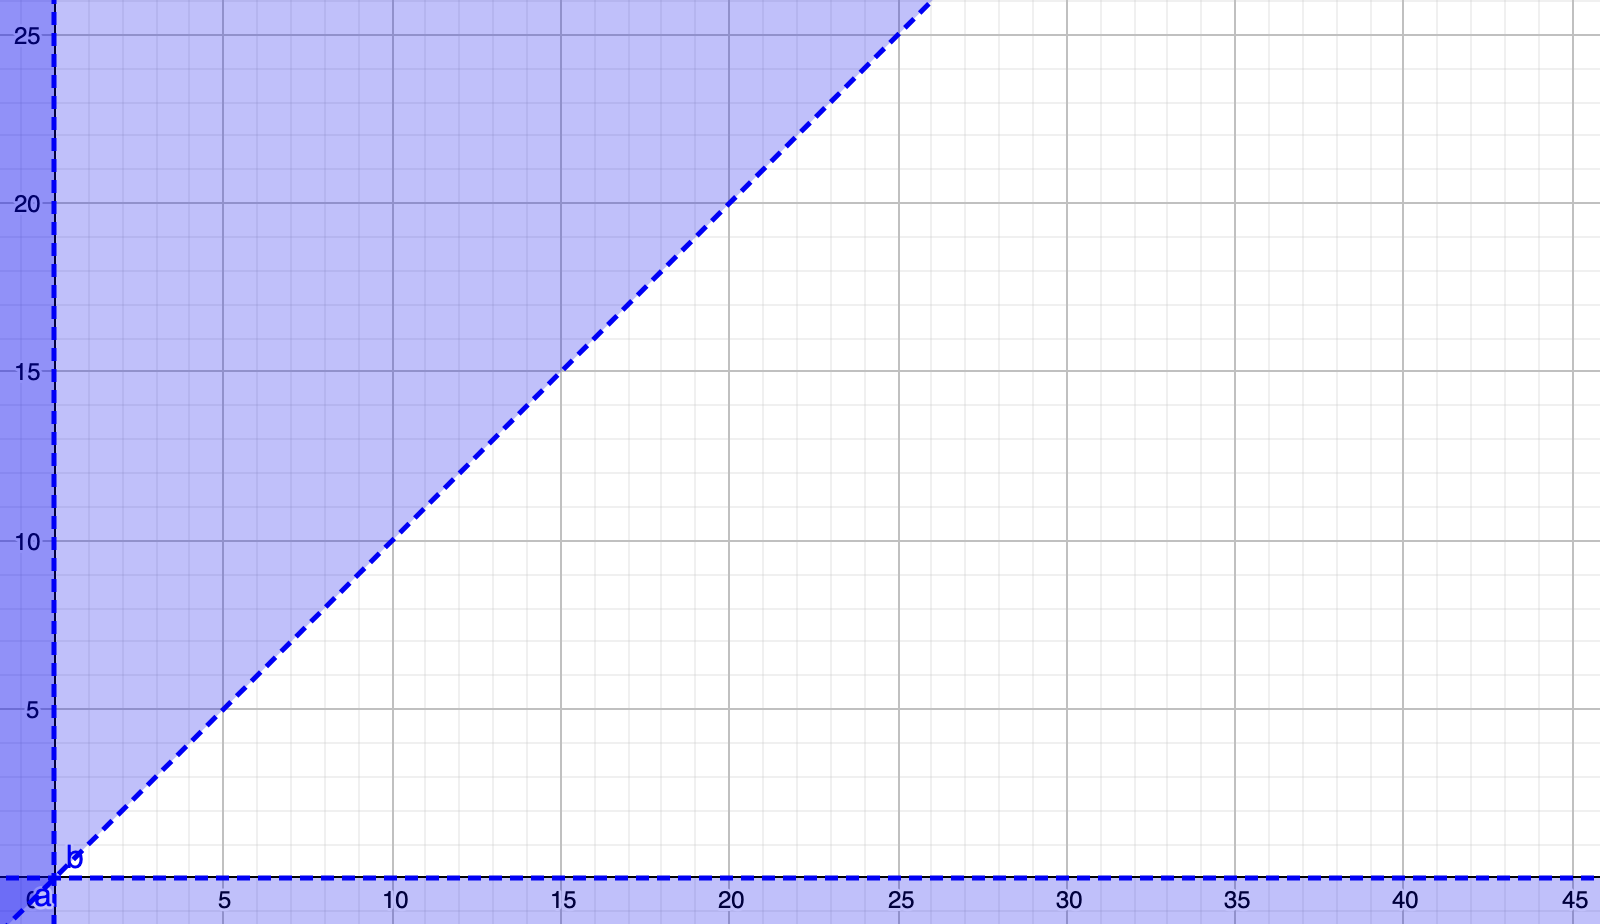
\includegraphics[width=0.8\textwidth]{assets/feasible_set_bigger_than.png}
    \caption{Sketch of the feasible set for $\beta \geq 0$ (the white area)}
  \end{figure}

  \begin{figure}[H]
    \centering
    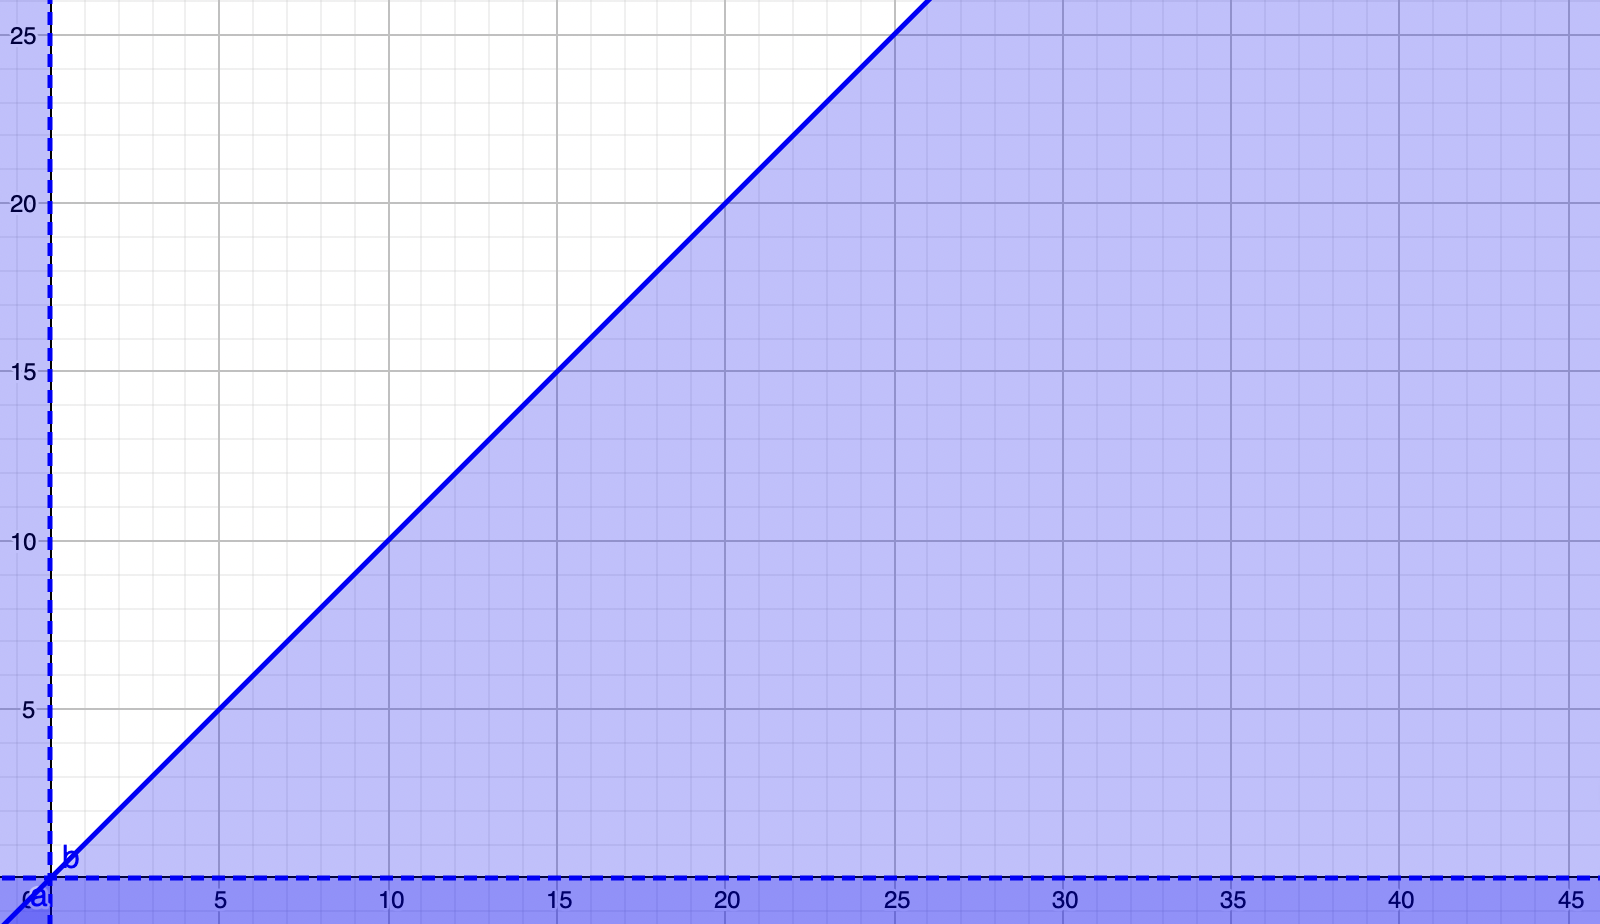
\includegraphics[width=0.8\textwidth]{assets/feasible_set_lower_than.png}
    \caption{Sketch of the feasible set for $\beta < 0$ (the white area)}
  \end{figure}

\end{enumerate}

For larger dimensions  \(n\), \(m\) the idea of transforming~\eqref{prob:sparse} into a linear optimization problem by introducing nonnegative and nonpositive parts of the solution remains valid.
That is, we put
\[
\tilde{x} = \begin{bmatrix}x^+\\x^-\end{bmatrix}\in\mathbb{R}^{2n},\qquad
\tilde{c} = \begin{bmatrix}1\\\vdots\\1\end{bmatrix}\in\mathbb{R}^{2n},\qquad
\qquad
\tilde{A} = \begin{bmatrix}
A & -A
\end{bmatrix},
\]
where the vectors \(x^+\in \mathbb{R}^n\), \(x^-\in \mathbb{R}^n\).
Then~\eqref{prob:sparse} is equivalent with a linear optimization problem:
\begin{equation}\label{prob:LP2}\begin{aligned}
&\text{minimize} && \tilde{c}\cdot \tilde{x},\\
&\text{subject to}&&\\
&&&\tilde{A}\tilde{x}= b,\\
&&& \tilde{x}\geq 0.
\end{aligned}\end{equation}

Throughout the following questions we will consider the particular instance of~\eqref{prob:LP2} where \(m=1\), \(n=5\), \(A=[1,2,3,4,5]\), and \(b = [10]\), from which one determines \(\tilde{A}\).
\begin{enumerate}
  \setcounter{enumi}{2}
  \item\label{spm:basic}
  Determine all \(10\) basic solutions for~\eqref{prob:LP2}, and select out of them \(5\) feasible basic solutions.
  (These solutions correspond to the extreme points/``corners'' of the \(10\)-dimensional feasible set for \(\tilde{x}\) and as such are not easy to visualize.) Evaluate the objective function in these 5 points and select the best one, which is thus a solution to~\eqref{prob:LP2}.
  \item[\textbf{Answer}] 
  \begin{align*}
    \tilde{A}\tilde{x}=b \\
    \begin{bmatrix}
      1 & 2 & 3 & 4 & 5 & -1 & -2 & -3 & -4 & -5
    \end{bmatrix}
    \tilde{x}=\begin{bmatrix}
      10
    \end{bmatrix}
  \end{align*}
  The 10 basic solutions are therefore:
  \begin{align*}
    \tilde{A}
  		\begin{bmatrix}
  			x_1 & 0 & 0 & 0 & 0 & 0 & 0 & 0 & 0 & 0
  		\end{bmatrix}^T
  		=
  		\begin{bmatrix}10\end{bmatrix},\qquad s_1=\begin{bmatrix}
  			\frac{10}{1} & 0 & 0 & 0 & 0 & 0 & 0 & 0 & 0 & 0
  		\end{bmatrix} \\
  		\tilde{A}
  		\begin{bmatrix}
  			0 & x_2 & 0 & 0 & 0 & 0 & 0 & 0 & 0 & 0
  		\end{bmatrix}^T
  		=
  		\begin{bmatrix}10\end{bmatrix},\qquad s_2=\begin{bmatrix}
  			0 & \frac{10}{2} & 0 & 0 & 0 & 0 & 0 & 0 & 0 & 0
  		\end{bmatrix} \\
  		\tilde{A}
  		\begin{bmatrix}
  			0 & 0 & x_3 & 0 & 0 & 0 & 0 & 0 & 0 & 0
  		\end{bmatrix}^T
  		=
  		\begin{bmatrix}10\end{bmatrix},\qquad s_3=\begin{bmatrix}
  			0 & 0 & \frac{10}{3} & 0 & 0 & 0 & 0 & 0 & 0 & 0
  		\end{bmatrix} \\
  		\tilde{A}
  		\begin{bmatrix}
  			0 & 0 & 0 & x_4 & 0 & 0 & 0 & 0 & 0 & 0
  		\end{bmatrix}^T
  		=
  		\begin{bmatrix}10\end{bmatrix},\qquad s_4=\begin{bmatrix}
  			0 & 0 & 0 & \frac{10}{4} & 0 & 0 & 0 & 0 & 0 & 0
  		\end{bmatrix} \\
  		\tilde{A}
  		\begin{bmatrix}
  			0 & 0 & 0 & 0 & x_5 & 0 & 0 & 0 & 0 & 0
  		\end{bmatrix}^T
  		=
  		\begin{bmatrix}10\end{bmatrix},\qquad s_5=\begin{bmatrix}
  			0 & 0 & 0 & 0 & \frac{10}{5} & 0 & 0 & 0 & 0 & 0
  		\end{bmatrix} \\
  		\tilde{A}
  		\begin{bmatrix}
  			0 & 0 & 0 & 0 & 0 & x_6 & 0 & 0 & 0 & 0
  		\end{bmatrix}^T
  		=
  		\begin{bmatrix}10\end{bmatrix},\qquad s_6=\begin{bmatrix}
  			0 & 0 & 0 & 0 & 0 & \frac{10}{-1} & 0 & 0 & 0 & 0
  		\end{bmatrix} \\
  		\tilde{A}
  		\begin{bmatrix}
  			0 & 0 & 0 & 0 & 0 & 0 & x_7 & 0 & 0 & 0
  		\end{bmatrix}^T
  		=
  		\begin{bmatrix}10\end{bmatrix},\qquad s_7=\begin{bmatrix}
  			0 & 0 & 0 & 0 & 0 & 0 & \frac{10}{-2} & 0 & 0 & 0
  		\end{bmatrix} \\
  		\tilde{A}
  		\begin{bmatrix}
  			0 & 0 & 0 & 0 & 0 & 0 & 0 & x_8 & 0 & 0
  		\end{bmatrix}^T
  		=
  		\begin{bmatrix}10\end{bmatrix},\qquad s_8=\begin{bmatrix}
  			0 & 0 & 0 & 0 & 0 & 0 & 0 & \frac{10}{-3} & 0 & 0
  		\end{bmatrix} \\
  		\tilde{A}
  		\begin{bmatrix}
  			0 & 0 & 0 & 0 & 0 & 0 & 0 & 0 & x_9 & 0
  		\end{bmatrix}^T
  		=
  		\begin{bmatrix}10\end{bmatrix},\qquad s_9=\begin{bmatrix}
  			0 & 0 & 0 & 0 & 0 & 0 & 0 & 0 & \frac{10}{-4} & 0
  		\end{bmatrix} \\
  		\tilde{A}
  		\begin{bmatrix}
  			0 & 0 & 0 & 0 & 0 & 0 & 0 & 0 & 0 & x_{10}
  		\end{bmatrix}^T
  		=
  		\begin{bmatrix}10\end{bmatrix},\qquad s_{10}=\begin{bmatrix}
  			0 & 0 & 0 & 0 & 0 & 0 & 0 & 0 & 0 & \frac{10}{-5}
  		\end{bmatrix} \\
  \end{align*}
  $s_6, s_7, s_8, s_9, s_{10}$ are not feasible solutions because they contains negative entries. Therefore the remaining $s_1, s_2, s_3, s_4, s_5$ are feasible solutions with the best solution being $s_5$ because: \[\frac{10}{5} < \frac{10}{4} < \frac{10}{3} < \frac{10}{2} < \frac{10}{1}\]
\item\label{spm:canonic}
Convert the problem~\eqref{prob:LP2} to a linear optimization problem in the canonical form.
\item[\textbf{Answer}] Converted to canonical form:
\begin{align*}
  \begin{aligned}
    &\text{maximize} && -\tilde{c}\cdot \tilde{x},\\
    &\text{subject to}&&\\
    &&&\tilde{A}\tilde{x} \leq b,\\
    &&&-\tilde{A}\tilde{x} \leq -b, \\
    &&& \tilde{x}\geq 0.
  \end{aligned}
\end{align*}
\item\label{spm:dual}
Write down the dual problem for the linear optimization problem in the canonical form obtained in the previous question.
Sketch the feasible set for the dual problem and solve it graphically.
Do you obtain the same optimal value for the objective function as in question~\ref{spm:basic}?
\item[\textbf{Answer}] 
\begin{align*}
  \begin{aligned}
    &\text{minimize} && b\cdot y_1-b \cdot y_2,\\
    &\text{subject to}&&\\
    &&&\begin{bmatrix}\tilde{A} \\ -\tilde{A}\end{bmatrix}^Ty \geq -\tilde{c}\\
    &&& y \geq 0.
  \end{aligned}
\end{align*}
The feasible set sketched is:
\begin{align*}
  \begin{aligned}
    &\text{minimize} && \begin{bmatrix}10\end{bmatrix} \cdot y_1-\begin{bmatrix}10\end{bmatrix}  \cdot y_2,\\
    &\text{subject to}&&\\
    &&& \begin{bmatrix}
      1 & -1 \\ 2 & -2 \\ 3 & -3 \\ 4 & -4 \\ 5 & -5 \\ -1 & 1 \\ -2 & 2 \\ -3 & 3 \\ -4 & 4 \\ -5 & 5
    \end{bmatrix}y \geq \begin{bmatrix}
      -1 \\-1 \\-1 \\-1 \\-1 \\-1 \\-1 \\-1 \\-1 \\-1
    \end{bmatrix} \\
    &&& y \geq 0.
  \end{aligned}
\end{align*}

\begin{figure}[htb]
  \centering
  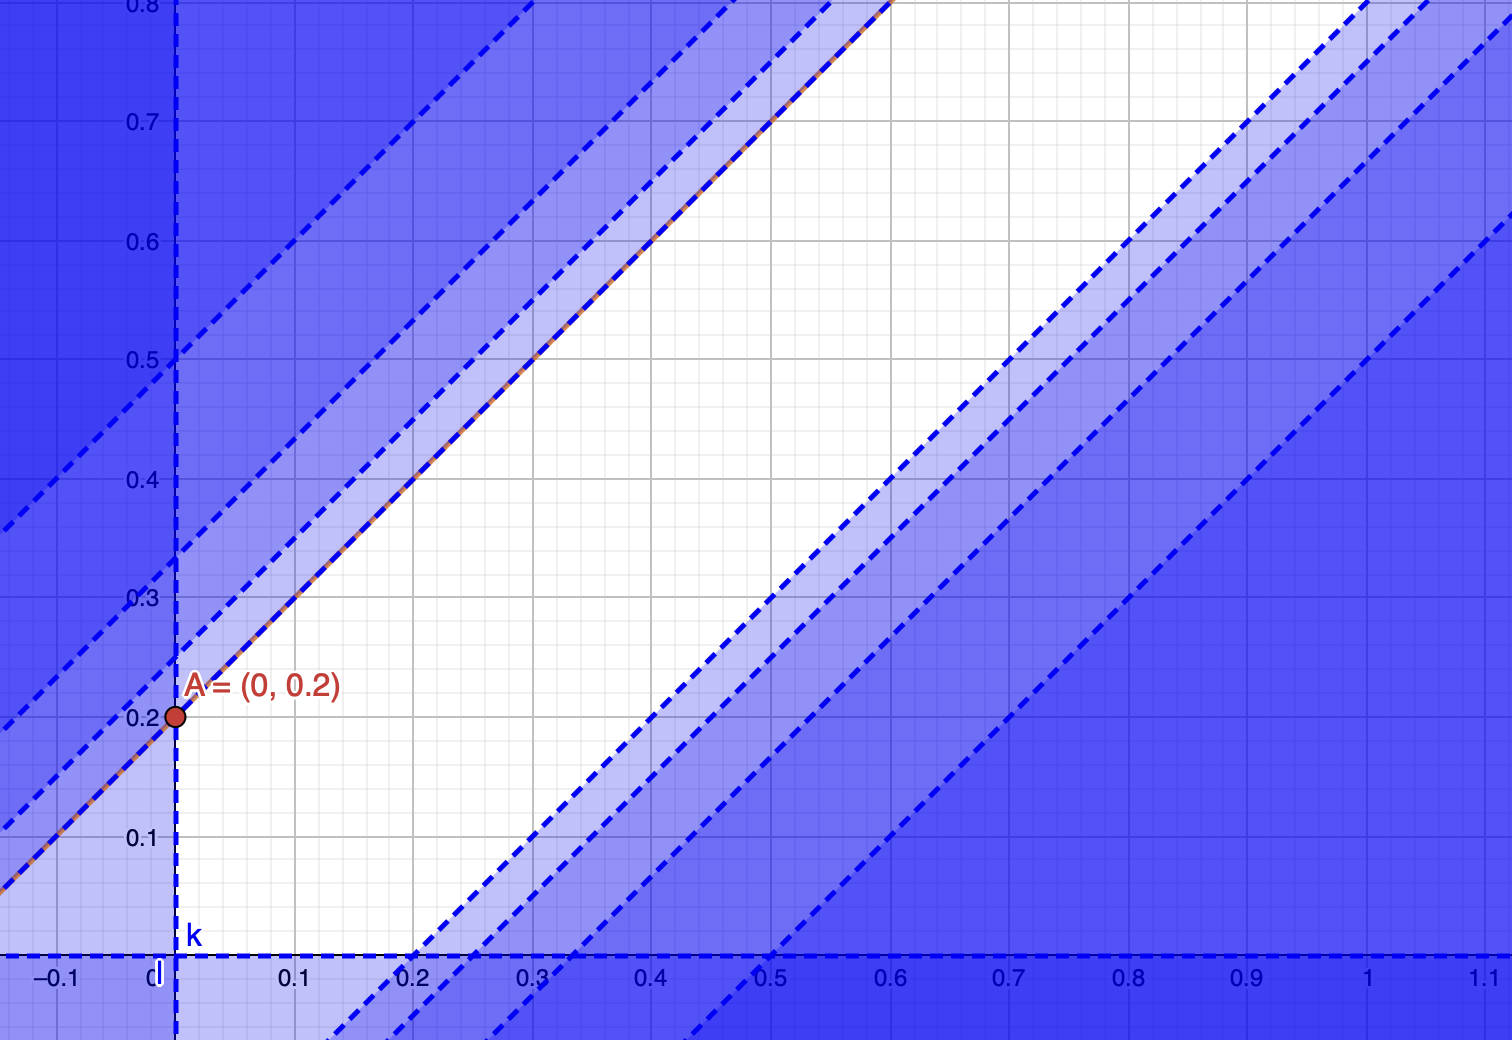
\includegraphics[width=0.8\textwidth]{assets/feasible_set_exercise_5.png}
\end{figure}

We obtain the value $10 \cdot 0 - 10 \cdot 0.2 = -2$. So the maximum value of the inverted problem is $-2$. This is consistent with the answer in question 3 because $-(-2)=2$. \\In question 4 we are converting the minimization problem to a maximization problem by inverting it. We are solving this maximization problem using the dual problem algorithm. Hence we will find the maximum of the inverted which $-2$. Therefore this solution it is consistent with the solution in question 3. 

\item Apply the simplex algorithm to solve the linear optimization problem in the canonical form from question~\ref{spm:canonic}.\footnote{Look at example 7 in section 9.3 [Lay] to see how to do this.}
Relate the computed optimal solution/objective value to the ones previously obtained in questions~\ref{spm:basic} and~\ref{spm:dual}.
Does the strong duality hold?
\item[\textbf{Answer}]
\begin{align*}
  \begin{array}{c}
    \\ 
    s_1 \\
    s_2 \\ 
    M
    \end{array}
    \begin{bmatrix}
    \begin{array}{ccccccccccccc|c}
      x_1 & x_2 & x_3 & x_4 & x_5 & x_6 & x_7 & x_8 & x_9 & x_{10} & s_1 & s_2 & M & b \\ \hline
      1 & 2 & 3 & 4 & 5 & -1 & -2 & -3 & -4 & -5 & 1 & 0 & 0 & 10  \\
      -1 & -2 & -3 & -4 & -5 & 1 & 2 & 3 & 4 & 5 & 0 & 1 & 0 & -10 \\ \hline
      1 & 1 & 1 & 1 & 1 & 1 & 1 & 1 & 1 & 1 & 0 & 0 & 1 & 0 \\
    \end{array}
  \end{bmatrix}
\end{align*}

As $s_2$ is negative, this is not yet a feasible solution. Because $\frac{-10}{-5}$ is the smallest nonnegative ratio we want to bring in $x_5$ into the solution.

\begin{align*}
  \begin{array}{c}
    \\ 
    s_1 \\
    x_5 \\ 
    M
    \end{array}
    \begin{bmatrix}
    \begin{array}{ccccccccccccc|c}
      x_1 & x_2 & x_3 & x_4 & x_5 & x_6 & x_7 & x_8 & x_9 & x_{10} & s_1 & s_2 & M & b \\ \hline
      0 & 0 & 0 & 0 & 0 & 0 & 0 & 0 & 0 & 0 & 1 & 1 & 0 & 0 \\
      \frac{1}{5} & \frac{2}{5} & \frac{3}{5} & \frac{4}{5} & 1 & \frac{-1}{5} & \frac{-2}{5} & \frac{-3}{5} & \frac{-4}{5} & -1 & 0 & \frac{-1}{5} & 0 & 2 \\ \hline
      \frac{4}{5} & \frac{3}{5} & \frac{2}{5} & \frac{1}{5} & 0 & \frac{6}{5} & \frac{7}{5} & \frac{8}{5} & \frac{9}{5} & 2 & 0 & \frac{1}{5} & 1 & -2 \\
    \end{array}
  \end{bmatrix}
\end{align*}

We get the same value as in exercise 3 and 5 so we are good to go. Because we have converted it to a maximum problem we want to find the maximum of the inverted values which is $-2$.
%TODO TJEK FOR STRONG DUALITY?
\end{enumerate}


\section*{Application: compressed sensing}

Our objective is to represent a time-dependent signal \(f(t)\), which we sample at some discrete times \(t_1, t_2, \dots, t_m\), as a linear combination of a few ``basis functions'' \(g_1, g_2, \dots, g_n\), \(n\geq m\),
with unknown weights \(x_j\).
That is, we would like to fulfill the equations
\[
  f(t_i) = \sum_{j=1}^n x_j g_j(t_i), \qquad \forall i=1,\dots,m,
\]
in such a way that \(\sum_{j=1}^n |x_j|\) is as small as possible.

\begin{enumerate}
  \setcounter{enumi}{6}
  \item Formulate the compressed sensing problem in the form~\eqref{prob:sparse}.
  That is, express the matrix \(A\) in terms of \(g_j\) and \(t_i\), and the right hand side vector \(b\) in terms of \(f\) and \(t_i\),
  \(i=1,\dots,m\), \(j=1,\dots,n\).
  \item[\textbf{Answer}]
  \begin{align*}
    \begin{aligned}
      &\text{minimize\ }& \sum_{j=1}^n |x_j|,\\
      &\text{subject to\ }& \begin{bmatrix}
        g_1(t_1) & g_j(t_1) & \cdots & g_n(t_1) & -g_1(t_1) & -g_j(t_1) & \cdots & -g_n(t_1) \\
        \vdots & \vdots & \ddots & \vdots & \vdots & \vdots & \ddots & \vdots \\
        g_1(t_m) & g_j(t_m) & \cdots & g_n(t_m) & -g_1(t_m) & -g_j(t_m) & \cdots & -g_n(t_m) \\
      \end{bmatrix}x=\begin{bmatrix}
        f(t_1) \\
        \vdots \\
        f(t_m)
      \end{bmatrix}
    \end{aligned}
  \end{align*}
  \item
  The file \verb|data.txt| on moodle contains the times \(t_i\) (first column) and the measured signal values \(f(t_i)\) (second column).
  Solve the instance of the compressed sensing problem given by this data and the following \(n=60\) ``basis functions,'' which include polynomials up to degree \(19\) and trigonometric functions:
  \[
    g_j(t) = \begin{cases}
    \cos((j-1)\arccos(t)), &\quad j=1,\dots,20, \quad\text{(Chebyshev polynomials)}\\
    \cos(\pi (j-20) t), &\quad j=21,\dots,40,\\
    \sin(\pi (j-40) t), &\quad j=41,\dots,60.
  \end{cases}
  \]
  Is the obtained representation of the signal/optimal solution to the problem ``compressed''/contains many zeros?
  Plot the data and the computed reconstruction of the signal.

  Hint: There are examples on moodle on how to read data files, solve linear probems of the type~\eqref{prob:LP2}, and plotting the results in Matlab and Python.
  \item[\textbf{Svar}] Yes, the optimal solution to the problem is "compressed" and contains many zeros. The problem is to minimize the sum of all $x$'s which is what we have done, and therefore the solution contians many zeros. The optimal solution with the following $x$ values in $\mathbb{R}^{120}$ is:
  \begin{align*}
    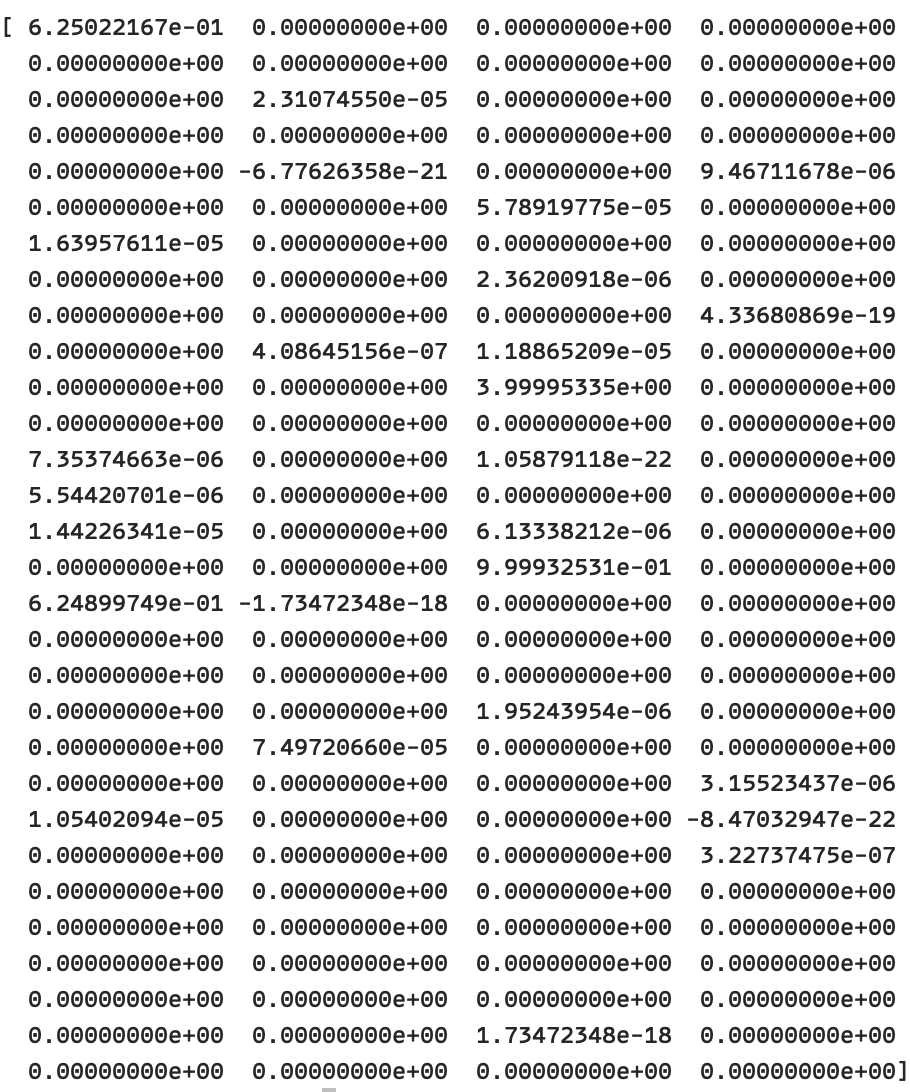
\includegraphics[width=0.5\textwidth]{assets/compressed_solution_x.png} \\
  \end{align*}
  And the solution visually with these $x$ values is:
  \begin{align*}
    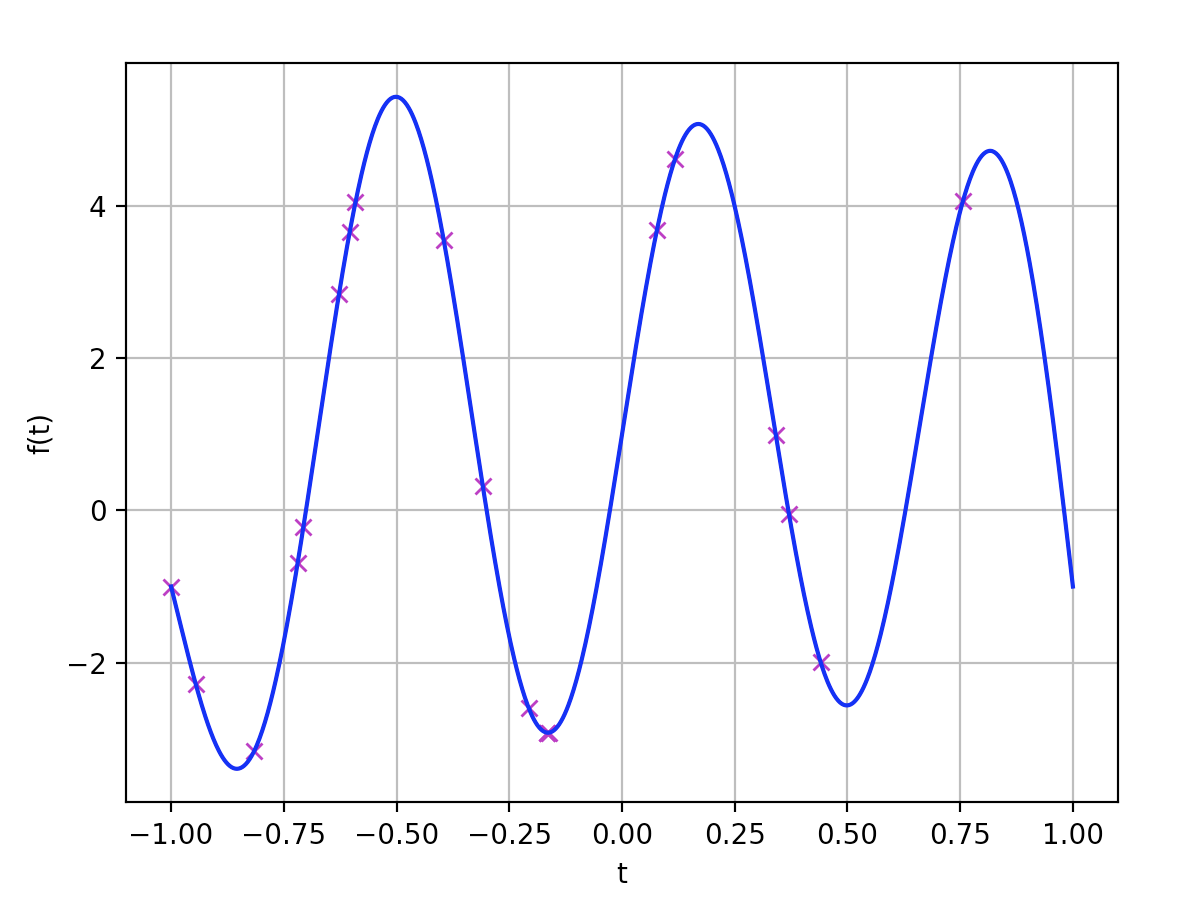
\includegraphics[width=0.5\textwidth]{assets/compressed_solution.png}
  \end{align*}
  The following code is how this solutions is found:
  \lstinputlisting[language=Python]{./assets/ws4-exercise8-solution.py}
\end{enumerate}
\end{document}
